\begin{frame}{Binäres One-Time-Pad (Bin-OTP)}
	Beim \textbf{Bin-OTP} arbeiten wir nicht mit dem lateinischen Alphabet $\{A, \dots, Z\}$, sondern mit dem binären Alphabet $\{0, 1\}$.
	
	\begin{figure}[H]
		\centering
		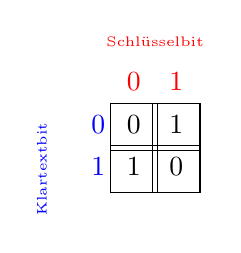
\begin{tikzpicture}[scale=0.9]
			\foreach \i in {0,...,1} {
				\node at (-0.5,-\i*0.6) {\textcolor{Blue}{\strut \i}};
				\node at (\i*0.6,0.6) {\textcolor{Red}{\strut \i}};
				\foreach \j in {0,...,1} {
					\edef\k{\ifnum\numexpr\i+\j\relax>1
							\the\numexpr\i+\j-2\relax
						\else
							\the\numexpr\i+\j\relax
						\fi}
					\node[draw,minimum size=0.6cm,inner sep=0pt]
					at (\i*0.6,-\j*0.6) {\strut\k};
				}
			}
			\node at (0.3,1.2) {\tiny{\textcolor{Red}{Schlüsselbit}}};
			\node[rotate = 90] at (-1.3,-0.6) {\tiny{\textcolor{Blue}{Klartextbit}}};
		\end{tikzpicture}
		\caption{Binäre Vigenère-Tabelle ($\oplus$ / XOR-Operation)}
	\end{figure}
\end{frame}

\begin{frame}{Verschlüsselung mit der $\oplus$-Operation (XOR)}
	Die Verschlüsselung erfolgt Bit für Bit mittels der Operation $\oplus$ (auch \emph{XOR} oder exklusives ODER genannt):
	\begin{align*}
		0 \oplus 0 = 0 \qquad\text{und}\qquad 0 \oplus 1 = 1 \\
		1 \oplus 0 = 1 \qquad\text{und}\qquad 1 \oplus 1 = 0
	\end{align*}\pause
	
	\begin{myexample}[Verschlüsselungsbeispiel]
		Klartext $\textcolor{Blue}{101}$, Schlüssel $\textcolor{ForestGreen}{111}$:
		\begin{center}
			\begin{tabular}{cccc}
				       & \textcolor{Blue}{1}        & \textcolor{Blue}{0}        & \textcolor{Blue}{1}        \\
				\oplus & \textcolor{ForestGreen}{1} & \textcolor{ForestGreen}{1} & \textcolor{ForestGreen}{1} \\
				\hline
				       & \textcolor{Red}{0}         & \textcolor{Red}{1}         & \textcolor{Red}{0}
			\end{tabular}
		\end{center}
		Somit ist der Kryptotext $\textcolor{Red}{010}$.
	\end{myexample}
\end{frame}

\begin{frame}{Mathematische Eigenschaften der $\oplus$-Operation}
	Für beliebige binäre Folgen $a, b, c$ gleicher Länge gelten folgende Gesetze:
	
	\begin{itemize}[<+->]
		\item \textbf{Kommutativität}: 
		      \[ a \oplus b = b \oplus a \]
		\item \textbf{Selbstinversität} (Verschlüsselung mit sich selbst ergibt $0$): 
		      \[ a \oplus a = 0 \]
		\item \textbf{Neutrales Element} (Verschlüsselung mit Nullen verändert nichts): 
		      \[ a \oplus 0 = a \]
		\item \textbf{Assoziativität}: 
		      \[ (a \oplus b) \oplus c = a \oplus (b \oplus c) \]
	\end{itemize}
\end{frame}

\begin{frame}{Warum funktioniert die Entschlüsselung?}
	Sei $t$ der Klartext und $s$ ein zufälliger geheimer Schlüssel.
	
	\begin{itemize}[<+->]
		\item \textbf{Verschlüsselung}: $c = t \oplus s$
		\item \textbf{Entschlüsselung} (erneute Anwendung desselben Schlüssels $s$):
		      \begin{align*}
			      c \oplus s & = (t \oplus s) \oplus s \\
			                 & = t \oplus (s \oplus s) \quad \text{(Assoziativität)} \\
			                 & = t \oplus 0 \qquad\quad \text{(Selbstinversität: } s \oplus s = 0\text{)} \\
			                 & = t \qquad\qquad\quad \text{(Neutrales Element: } t \oplus 0 = t\text{)}
		      \end{align*}
	\end{itemize}
	\pause
	Die erneute Anwendung des Schlüssels hebt die Verschlüsselung vollständig auf!
\end{frame}

\begin{frame}{Auftrag: Bin-OTP}
	\begin{itemize}
		\item \aufgabebox{Aufgaben 2.18-2.21}
		\item Zeit: 15 Minuten
		\item Danach: Gemeinsame Besprechung der Lösungen
	\end{itemize}
\end{frame}
